\documentclass[border=10pt]{standalone}
\usepackage{tikz}\usepackage{amsmath}\usetikzlibrary{matrix,arrows.meta}
\begin{document}
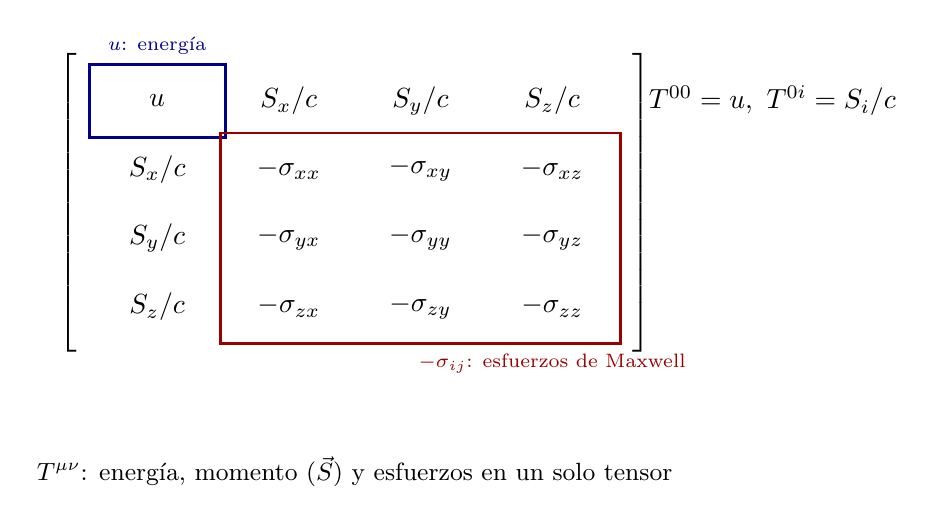
\begin{tikzpicture}[line width=0.8pt]
  \matrix (T) [matrix of math nodes, left delimiter={[}, right delimiter={]},
     nodes={minimum width=1.7cm,minimum height=0.9cm,anchor=center},
     row sep=-\pgflinewidth, column sep=-\pgflinewidth]{
    u & S_x/c & S_y/c & S_z/c \\
    S_x/c & -\sigma_{xx} & -\sigma_{xy} & -\sigma_{xz} \\
    S_y/c & -\sigma_{yx} & -\sigma_{yy} & -\sigma_{yz} \\
    S_z/c & -\sigma_{zx} & -\sigma_{zy} & -\sigma_{zz} \\
  };
  \draw[blue!55!black,line width=1pt] (T-1-1.north west) rectangle (T-1-1.south east);
  \draw[red!60!black,line width=1pt] (T-2-2.north west) rectangle (T-4-4.south east);
  \node[blue!55!black,anchor=south] at (T-1-1.north){\scriptsize $u$: energía};
  \node[red!60!black,anchor=north] at (T-4-4.south){\scriptsize $-\sigma_{ij}$: esfuerzos de Maxwell};
  \node[anchor=west] at (T-1-4.east) {\ \ $T^{00}=u,\ T^{0i}=S_i/c$};
  \node at (0,-3.4){\small $T^{\mu\nu}$: energía, momento ($\vec S$) y esfuerzos en un solo tensor};
\end{tikzpicture}
\end{document}
